%!TEX program = xelatex
\documentclass[a4paper,12pt]{report}
\usepackage{indentfirst} 
\usepackage{ctex}
%\usepackage{xeCJK}
\usepackage{times}
\usepackage{graphicx,float}
\usepackage{setspace}
\usepackage{fancyhdr}
% \usepackage{graphicx}
\usepackage{wrapfig}
\usepackage{array}
\usepackage{fontspec,xunicode,xltxtra}
\usepackage{titlesec}
\usepackage{titletoc}
\usepackage[titletoc]{appendix}
\usepackage[top=30mm,bottom=30mm,left=20mm,right=20mm]{geometry}
\usepackage{cite}
\usepackage{listings}
\usepackage[framed,numbered,autolinebreaks,useliterate]{mcode} % 插入代码
\XeTeXlinebreaklocale "zh"
\XeTeXlinebreakskip = 0pt plus 1pt minus 0.1pt

%---------------------------------------------------------------------
%	页眉页脚设置
%---------------------------------------------------------------------
\fancypagestyle{plain}{
	\pagestyle{fancy}      %改变章节首页页眉
}

\pagestyle{fancy}
\lhead{\kaishu~``计算机网络''实验报告~}
\rhead{\kaishu~~实验1}
\cfoot{\thepage}

%---------------------------------------------------------------------
%	章节标题设置
%---------------------------------------------------------------------
\titleformat{\chapter}{\centering\zihao{-1}\heiti}{实验\chinese{chapter}}{1em}{}
\titlespacing{\chapter}{0pt}{*0}{*6}

%---------------------------------------------------------------------
%	摘要标题设置
%---------------------------------------------------------------------
\renewcommand{\abstractname}{\zihao{-3} 摘\quad 要}

%---------------------------------------------------------------------
%	参考文献设置
%---------------------------------------------------------------------
\renewcommand{\bibname}{\zihao{2}{\hspace{\fill}参\hspace{0.5em}考\hspace{0.5em}文\hspace{0.5em}献\hspace{\fill}}}

%---------------------------------------------------------------------
%	引用文献设置为上标
%---------------------------------------------------------------------
\makeatletter
\def\@cite#1#2{\textsuperscript{[{#1\if@tempswa , #2\fi}]}}
\makeatother

%---------------------------------------------------------------------
%	目录页设置
%---------------------------------------------------------------------
\titlecontents{chapter}[0em]{\songti\zihao{-4}}{\thecontentslabel\ }{}
{\hspace{.5em}\titlerule*[4pt]{$\cdot$}\contentspage}
\titlecontents{section}[2em]{\vspace{0.1\baselineskip}\songti\zihao{-4}}{\thecontentslabel\ }{}
{\hspace{.5em}\titlerule*[4pt]{$\cdot$}\contentspage}
\titlecontents{subsection}[4em]{\vspace{0.1\baselineskip}\songti\zihao{-4}}{\thecontentslabel\ }{}
{\hspace{.5em}\titlerule*[4pt]{$\cdot$}\contentspage}

\renewcommand\thesection{\arabic{section}}
\renewcommand\thesubsection{\arabic{section}.\arabic{subsection}}

\begin{document}
%---------------------------------------------------------------------
%	封面设置
%---------------------------------------------------------------------
\begin{titlepage}
	\begin{center}
		
    
\includegraphics[width=1.0\textwidth]{figure//nankai.jpg}\\
    % \vspace{10mm}
    % \textbf{\zihao{2}\kaishu{软件学院}}\\[0.8cm]
    \vspace{50mm}
    \textbf{\zihao{1}\heiti{ 《计算机网络》实验报告}}\\[1cm]
    \textbf{\zihao{2}\heiti{ (2022\textasciitilde2023学年第一学期)}}\\[1cm]
    %\textbf{\zihao{2}\heiti{ 实验1: Wireshark 软件使用\\ 与ARP 协议分析}}\\[2cm]
	\vspace{\fill}
	
\setlength{\extrarowheight}{2mm}
{\songti\zihao{3}	
\begin{tabular}{rl}

	{\makebox[4\ccwd][s]{实验名称:}}& ~\kaishu Wireshark软件使用\\
	{\makebox[4\ccwd][s]{学\qquad 院:}}& ~\kaishu 软件学院\\
		{\makebox[4\ccwd][s]{姓\qquad 名:}}& ~\kaishu 张三\\

    {\makebox[4\ccwd][s]{学\qquad 号:}}& ~\kaishu 001~002~003 \\

	{\makebox[4\ccwd][s]{指导老师:}} & ~\kaishu 张圣林\\

\end{tabular}
 }\\[2cm]
\vspace{\fill}
\zihao{4}
%2021\textasciitilde 2022秋季学期\\
%使用\LaTeX 撰写于
    \today
	\end{center}	
\end{titlepage}


%---------------------------------------------------------------------
%  目录页
%---------------------------------------------------------------------
\tableofcontents % 生成目录

%---------------------------------------------------------------------
%  实验一
%---------------------------------------------------------------------
\chapter*{实验名称(实验1:Wireshark软件使用
)}
\setcounter{page}{1}
\begin{spacing}{1.5}
\songti\zihao{-4}

%\section{分工情况}
 %\begin{itemize}
 %	\item 张三:
 %	\item 李四:
 %	\item 六六:
 %\end{itemize}
\section{实验目的}
通过学习 ...,掌握 ...

\section{实验条件}
该实验所使用的环境、工具 ...

\section{实验报告内容及原理}
根据实验要求,写出该实验具体步骤内容...,可涉及实验原理、方法及手段等进行相关分析。


\section{实验结论及心得体会}
通过这次实验记录自己在本次实验中所遇到的问题,以及心得感悟即相关问题和解决方法。如果遇到异常情况,或者无法完成任务时,也请分析错误产生的原因。

\end{spacing}

\section{代码截图}
\zihao{-4}\songti
\begin{spacing}{1.5}
代码/过滤语法的实验截图如图~\ref{pic1}所示\\
\indent\setlength\parindent{2em}(进行分析实验数据报文的相关截图)

\begin{figure}[htb]
  \centering
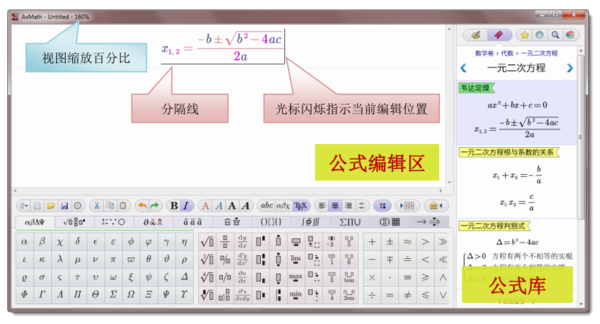
\includegraphics[width=12cm]{figure/calculator.png}\caption{计算器截图}\label{pic1}
\end{figure}


代码/过滤语法的实验截图如图~\ref{pic2}所示\\
\indent\setlength\parindent{2em}(进行分析实验数据报文的相关截图)

\begin{figure}[htb]
  \centering
\includegraphics[width=12cm]{figure/pic2.png}\caption{MAC地址}\label{pic2}
\end{figure}

\end{spacing}



\section{核心代码/核心过滤语法}
\zihao{-4}\songti
\begin{spacing}{1.5}
核心代码/核心过滤语法如下:

\subsubsection{代码GitHub地址 (此项可有可无,具体根据每个实验要求)} 
软件的GitHub地址为

\end{spacing}


%---------------------------------------------------------------------
%  参考文献设置
%---------------------------------------------------------------------
% \addcontentsline{toc}{chapter}{参考文献}

% \begin{thebibliography}{99}
% \songti \zihao{-4} 	
% 	\bibitem{Leslie.{1994}}
% 	Leslie Lamport. LATEX: A Document Preparation System.AddisonWesley, Reading, Massachusetts, second edition, 1994, ISBN 0-201-52983-1.
	
% 	\bibitem{Donald.{1984}}
% 	Donald E. Knuth. The TEXbook, Volume A of Computers and Typesetting,Addison Wesley, Reading, Massachusetts, second edition, 1984,ISBN 0-201-13448-9.

	
% \end{thebibliography}

%---------------------------------------------------------------------
%  附录设置
%---------------------------------------------------------------------
% \titleformat{\chapter}{\heiti\Large}{附录~\Alph{chapter}}{11pt}{\Large}
% \titlespacing{\chapter}{0pt}{*-4}{*4}

% \lstset{breaklines}                %自动将长的代码行换行排版
% \lstset{extendedchars=false}
% \lstset{language=Matlab}
% \renewcommand{\thechapter}{附录\Alph{chapter}.}
% \appendix
% \begin{appendix}
	
	

% \end{appendix}
		

\end{document}
